\documentclass[tikz,border=10pt]{standalone}
\usepackage{amsmath}
\usepackage{amssymb}
\usepackage{tikz}
\usetikzlibrary{arrows.meta,calc}

\definecolor{figazul}{RGB}{2,132,199}
\definecolor{figrojo}{RGB}{220,38,38}
\definecolor{figverde}{RGB}{22,163,74}

\begin{document}
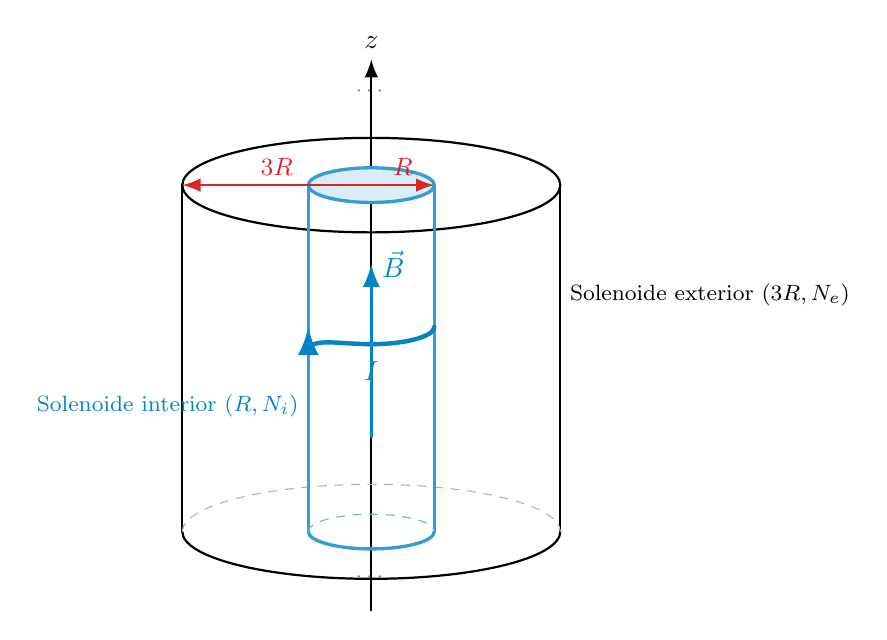
\begin{tikzpicture}[>=Latex, line cap=round, line join=round]
  % Eje vertical z
  \draw[->, thick] (0, -3.2) -- (0, 3.8) node[above] {$z$};

  % Solenoide exterior: radio 3R = 2.4, altura de z = -2.2 a +2.2
  % Elipse superior exterior
  \draw[thick] (0, 2.2) ellipse (2.4 and 0.6);
  % Generatrices exteriores
  \draw[thick] (-2.4, -2.2) -- (-2.4, 2.2);
  \draw[thick] (2.4, -2.2) -- (2.4, 2.2);
  % Elipse inferior exterior: parte frontal continua, trasera discontinua
  \draw[thick] (2.4, -2.2) arc (0:-180:2.4 and 0.6);
  \draw[dashed, thin, color=gray!60] (-2.4, -2.2) arc (180:0:2.4 and 0.6);

  % Solenoide interior: radio R = 0.8, altura de z = -2.2 a +2.2
  % Generatrices interiores
  \draw[very thick, color=figazul!80] (-0.8, -2.2) -- (-0.8, 2.2);
  \draw[very thick, color=figazul!80] (0.8, -2.2) -- (0.8, 2.2);
  % Elipse superior interior
  \draw[very thick, color=figazul!80, fill=figazul!15] (0, 2.2) ellipse (0.8 and 0.22);
  % Elipse inferior interior
  \draw[very thick, color=figazul!80] (0.8, -2.2) arc (0:-180:0.8 and 0.22);
  \draw[dashed, thin, color=figazul!60] (-0.8, -2.2) arc (180:0:0.8 and 0.22);

  % Espiras / corriente en el solenoide interior (I en sentido antihorario)
  \draw[->, ultra thick, color=figazul] (0.8, 0.4) arc (0:-180:0.8 and 0.22) node[below=2pt, midway, color=figazul] {$I$};

  % Campo B confinado en el interior (r < R)
  \draw[->, very thick, color=figazul] (0, -1.0) -- (0, 1.2) node[right, color=figazul] {$\vec{B}$};

  % Cotas de radio en la elipse superior (en rojo)
  % Radio R del solenoide interior
  \draw[->, thick, color=figrojo] (0, 2.2) -- (0.8, 2.2);
  \node[above, color=figrojo, font=\small] at (0.4, 2.2) {$R$};

  % Radio 3R del solenoide exterior
  \draw[->, thick, color=figrojo] (0, 2.2) -- (-2.4, 2.2);
  \node[above, color=figrojo, font=\small] at (-1.2, 2.2) {$3R$};

  % Etiquetas de solenoides
  \node[right, font=\footnotesize] at (2.4, 0.8) {Solenoide exterior ($3R, N_e$)};
  \node[left, font=\footnotesize, color=figazul] at (-0.8, -0.6) {Solenoide interior ($R, N_i$)};

  % Indicación de longitud infinita
  \node[above, font=\footnotesize, color=gray] at (0, 3.2) {$\cdots$};
  \node[below, font=\footnotesize, color=gray] at (0, -2.6) {$\cdots$};
\end{tikzpicture}
\end{document}
